\documentclass[letterpaper, 10 pt, conference]{ieeeconf}
%\documentclass[a4paper, 10pt, conference]{ieeeconf}

\overrideIEEEmargins

\usepackage[utf8]{inputenc}
\usepackage[T1]{fontenc}
\usepackage{hyperref}
\usepackage{url}
\usepackage{graphicx}
\usepackage{ngerman}

\hypersetup{hidelinks}

\title{\LARGE
\textbf{FireForceDefense} \\ Technical Report
}

\author{Cameron Barbee, Tim Hoffmann,  Christian Piffel,  Tobias Schotter,\\  Sebastian Schuscha,  Philipp Stangl,  Thomas Stangl%
}

\begin{document}

\maketitle
\thispagestyle{empty}
\pagestyle{empty}

\section{Einführung und Ziele}

Im vorliegenden Projekt soll das Tower-Defense-Spiel „FireForceDefense“ erweitert werden.
Ziel ist es, das Spiel um eine einfache Benutzerverwaltung, d.h. Registrierung und Anmeldung, zu ergänzen.
Außerdem soll eine Rangliste geschaffen werden, wofür eine Spielstand-Speicherung notwendig ist.

\section{Bausteinsicht}
Diese Sicht zeigt die statische Zerlegung des Systems in Bausteine sowie
deren Beziehungen.  %\cite{c1}

\begin{figure}[thpb]
      \centering
      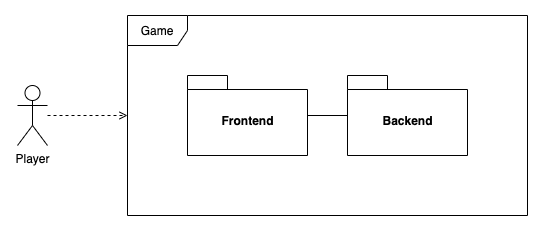
\includegraphics[scale=0.38]{images/context}
      \caption{Kontextabgrenzung}
      \label{fig:context}
\end{figure}


\subsection{Gesamtsystem}
%Whitebox-Beschreibung des Gesamtsystems,
%zusammen mit Blackbox-Beschreibungen der darin enthaltenen Bausteine.
Die Anwendung basiert auf einer Client-Server-Architektur (\ref{fig:context}).
Frontend und Backend kommunizieren über eine RESTful-API.


\subsection{Frontend}
Dieser Abschnitt beschreibt die client-seitige Frontend-Architektur.
Das Frontend wird unter Zuhilfenahme des Frameworks Vue.js realisiert.

Es ist selbst in mehrere Unter-Bausteine zerlegt:

\subsubsection{Model}

Dieser Baustein enthält die Logik für den Problembereich im Frontend.
Die eigentlichen Anzeigekomponenten besitzen Referenzen auf die Instanzen der Klassen des Model-Bereichs,
sodass Eingaben an das Model weitergegeben und dort verarbeitet werden können.
Schließlich besitzt das Model Schnittstellen, mittels denen Informationen über den aktuellen Zustand abgefragt werden können,
um basierend darauf die Anzeige anzupassen.

Im Model ist beispielsweise die Spiellogik und die Schnittstelle zum Speichern und Abrufen von Spielständen verortet.

\subsubsection{Components}

In diesem Modul sind die Vue-Komponenten gesammelt, mit denen die eigentliche Anzeige im Webbrowser realisiert wird.
Die Komponenten sind dabei hierarchisch geordnet, so besteht ein Level beispielsweise aus einer Sidebar und der LevelMap,
die LevelMap wiederum enthält einzelne Zellen und so weiter.

Die Komponenten behandeln alle Eingaben und senden bei Bedarf entsprechende Nachrichten an das Model.

\subsubsection{SCSS}

Hier werden zentral genutzte Stile im SCSS-Format abgelegt.

\subsubsection{Lang}

Dieser Baustein ist für die Internationalisierung, genauer gesagt die Übersetzung, zuständig.
Aktuell ist lediglich eine deutsche Sprachvariante hinterlegt.

\subsubsection{Levels}

Dieses Modul enthält die Level-Definitionen.
Eine Level-Definition beschreibt den initialen Aufbau des Spielfelds und die auftretenden Effekte.
Jedes Level muss anhand der jeweiligen Definition im LevelManager des Model-Bereichs registriert werden.

\subsubsection{Cells, Contents und Effects}

In diesen drei Bausteinen sind die verschiedenen, konkreten Zell-, Inhalts- bzw. Effekt-Typen samt ihren jeweiligen Eigenschaften hinterlegt.

\subsection{Backend}
Dieser Abschnitt beschreibt die server-seitige Backend-Architektur.

\subsubsection{Datenbank} \label{datenbank}

Die Speicherung der Daten erfolgt im dokumentenorientierten NoSQL-Datenbankmanagementsystem \textit{MongoDB}.
Zusätzlich wird die Bibliothek  \textit{mongoose} für das Object Data Modeling (ODM) verwendet. \\
Der folgende Teilbereich beschreibt die Unterteilung der Daten in drei Collection:

\begin{itemize}
\item
\textit{Accounts:} Hier werden die nötigen Informationen eines Benutzers gespeichert, um
eine Login- und Registrierungsfunktion zu gewährleisten. Das ist einerseits ein
einzigartiger Benutzername, eine E-Mailadresse, ein verschlüsseltes Passwort, sowie
ein Datum, welches den Registrierungszeitpunkt festhält.
\item
\textit{Refreshtokens:} In dieser Dokumentensammlung werden alle nötigen Informationen für
das Session-Handling gespeichert. Das ist einerseits die von MongoDB automatisch
erstellte ID der einzelnen Benutzer, um jedem Benutzer seinen entsprechenden Token
zuweisen zu können. Dazu wird der entsprechende Token gespeichert, sowie ein Verfallsdatum
des Tokens, ein Erstellungsdatum des Dokumentes und abschließend ein Wert, welcher die
IP des Erstellers festhält.
\item
\textit{Scores:} Diese Sammlung an Dokumenten speichert grundlegend alle relevanten Aspekte des
Spielstandes. Einerseits den Benutzernamen, das Level, die erreichten Sterne, das
übriggebliebene Geld, sowie die verwendete Zeit und die Anzahl an verbrannten Zellen.
Anhand dieser Informationen wird die Reihenfolge der Rangliste berechnet.
\end{itemize}

\subsubsection{Laufzeitumgebung}

JavaScript-basierte Plattform Node.js mit dem serverseitigen Webframework ExpressJS.

\section{Verteilungssicht}
Das Verteilungssicht beschreibt die Verteilung des Gesamtsystems,  wichtige Begründungen für diese Verteilungsstruktur und die Zuordnung von Softwareartefakten zu Bestandteilen der Infrastruktur.
Zentrale Bestandteile der Verteilungsstruktur sind (A) das Kubernetes Cluster,  (B) das Datenbank-Cluster und (C) die GitLab CI/CD-Pipeline.

\subsection{Kubernetes Cluster}

Für ein Kubernetes-Cluster wurde sich entschieden, aufgrund der Tatsache, das mehrere virtuelle Cluster (sog. Namespaces) auf demselben physischen Cluster unterstützt werden. Dadurch kann die CI/CD Pipeline im \textit{Gitlab-managed-apps} Namespace laufen, währenddessen die Anwendung auf einem anderen Namespace bereitgestellt wird.

Das Kubernetes Cluster wird über den Elastic Kubernetes Service des Cloud-Providers Amazon Web Services bereitgestellt.  Aus datenschutzrechtlichen Gründen werden nur Cloud Server, die der Verfügbarkeitszone Frankfurt (eu-central-1) angehörig sind, verwendet.

\subsection{Datenbank-Cluster}
Das Datenbank-Cluster besteht aus drei Replikationen. Es stellt jeweils eine Datenbank für den Entwicklungs- und Produktionsbetrieb bereit. Näheres zur Datenbank wird im Abschnitt \ref{datenbank} erklärt.

\begin{figure}[thpb]
      \centering
      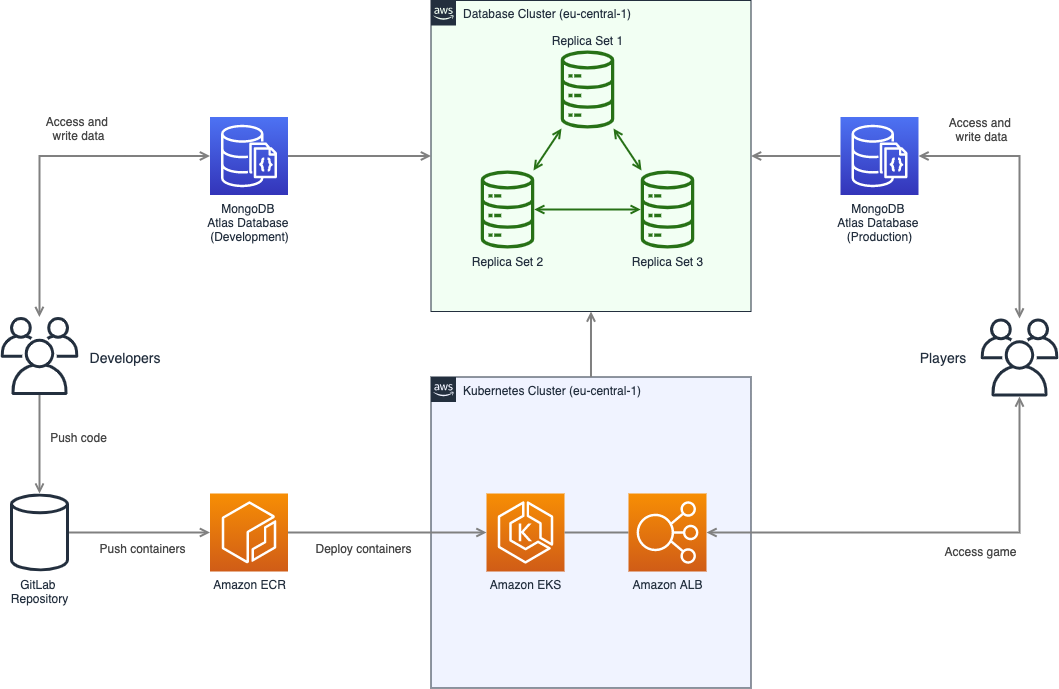
\includegraphics[scale=0.22]{images/infrastructure}
      \caption{Cloud Infrastruktur}
      \label{fig:infrastructure}
\end{figure}


\subsection{CI/CD-Pipeline}

Für die Bereitstellung der CI/CD Pipeline ist ein Kubernetes-Executor\cite{c1} auf dem Kubernetes Cluster verantwortlich.  Dieser verbindet sich mit der Kubernetes Cluster API und erstellt einen Pod für jeden GitLab CI Job. Dieser Pod besteht aus einem Build-Container und einem zusätzlichen Container für jeden Service. Die Pipeline umfasst das Erstellen, Testen und Bereitstellen der Anwendung.  Folgende vier Stages durchläuft jeder Push in das Gitlab-Repository:

\subsubsection{Dependencies}

Installation der npm-Pakete in das Verzeichnis node\_modules.

\subsubsection{Lint}

Durchführung statischer Code-Analysen.

\subsubsection{Build}

Alle notwendigen Bau-/Vorbereitungsaufgaben der Anwendung werden ausgeführt.

\subsubsection{Test}

Durchführung von Unit Tests, um die Korrektheit des Codes zu validieren.  \\

Die letzten beiden Stages werden nur im main-Zweig des Repositories durchlaufen, um die Anwendung für den Produktionsbetrieb bereitzustellen.

\subsubsection{Dockerize}

Wenn alle Unit Tests bestanden sind, wird für Front- und Backend jeweils ein Docker-Image gebaut. Anschließend werden beide Images im Docker-Registry abgelegt, damit sie für die nächste Stage (Deploy) verfügbar sind.

\subsubsection{Deploy}

In der letzten Phase werden die Docker Images aus der Docker-Registry auf dem Kubernetes Cluster als Container bereitgestellt. Die Anwendung ist dann,  bis einschließlich dem Tag der Präsentation, öffentlich zugänglich.


\section{Entwicklungsumgebung und Tools}

\subsection{IDE}

Das Projekt ist so ausgerichtet, dass es keine Beschränkung auf eine bestimmte IDE gibt.
Die meisten Teammitglieder verwenden JetBrains Phpstorm.

\subsection{Paketverwaltung}

Die Verwaltung der Abhängigkeiten erfolgt mit „npm“.

\subsection{Linting}

In beiden Unterprojekten (Frontend und Backend) wird jeweils „eslint“ in Verbindung mit „prettier“ verwendet,
um die Einhaltung der Codierrichtlinien zu gewährleisten.

Die Konfigurationen sind jeweils in den Dateien \texttt{eslintrc.js} und \texttt{prettierrc.js} hinterlegt.

\subsection{Build-Tools}

\subsubsection{Backend}

Im Backend wird der Typescript Compiler „tsc“ verwendet, um die Dateien in ein Format zu überführen,
welches mit \texttt{node} ausgeführt werden kann.

Die Konfiguration findet sich dabei in der Datei \texttt{tsconfig.json}.

\subsubsection{Frontend}

Im Frontend ist Webpack dafür zuständig, die Anwendung aus dem Quellcode zu erstellen.
Dabei gibt es zwei Varianten:
Für Entwicklungszwecke wird ein Webpack-Dev-Server (mit Reload-Funktionalität) zum Bereitstellen der Anwendung verwendet,
während für den Produktiveinsatz nur die benötigten Zieldateien erstellt werden, die dann mit einer beliebigen Server-Software ausgeliefert werden können.

Die Webpack-Konfiguration erfolgt in den \texttt{webpack.config.*.js}-Dateien.
Darin ist festgelegt, dass die CSS-Bestandteile in der Ausgabedatei \texttt{main.css} gesammelt werden.
Die Index-Datei und die Assets werden in das Ausgabeverzeichnis kopiert, die Vue-Single-File-Component-Dateien werden übersetzt
und Typescript wird zu JavaScript kompiliert.

Ferner sind Alias-Namen für häufig genutzte Verzeichnisse definiert, um Pfadangaben zu vereinfachen.

\subsection{Unit Tests}

Unit-Tests werden mit „Jest“ realisiert.
Snapshot-Tests für die Frontend-Komponenten sind dabei durch die Pakete „vue-jest“ und „vue-test-utils“ möglich.

\section{Detailinformationen}

Im Folgenden werden die beiden Bereiche „Session Handling“ und „Rangliste“, welche der Hauptfokus der diesjährigen Arbeiten waren, etwas genauer betrachtet.

\subsection{Session Handling}

TODO

\subsection{Rangliste}

Die Spielergebnisse werden nach der Beendigung eines jeden Levels als Dokument in der „scores“-Collection der MongoDB abgelegt.

Basierend darauf wird backendseitig eine GET-Schnittstelle bereitgestellt,
über welche – unter optionaler Angabe eines Levels, nach dem gefiltert werden soll – die aggregierten Spielstandsdaten abgefragt werden können.
Diese Aggregation führt dazu, dass es pro Benutzername einen Eintrag gibt, welcher die aufaddierte Gesamtzahl der erreichten Sterne,
die durchschnittlich benötigte Spieldauer, das durchschnittlich angesparte In-Game-Geld-Guthaben, sowie die durchschnittliche Anzahl der abgebrannten Felder enthält.

Auch die Sortierung erfolgt bereits im Backend, und zwar nach folgenden Kriterien (in absteigender Priorität geordnet):
Sternenanzahl (absteigend), Anzahl der verbrannten Felder (aufsteigend), Geld-Guthaben (absteigend) und Spielzeit (absteigend).

Im Frontend werden diese Daten durch eine HTTP-Anfrage beschafft und durch eine Vue-Komponente auf einer eigenen Seite angezeigt.
Dabei haben Benutzer*innen die Möglichkeit, entweder eine Gesamtansicht über alle Level hinweg oder eine nach einem bestimmten Level gefilterte Ansicht auszuwählen.

Die eigene Ranglisten-Position wird hervorgehoben und fixiert angezeigt.

\section{Querschnittliche Konzepte}

Dieser Abschnitt beschreibt übergreifende, prinzipielle Regelungen und
Lösungsansätze, die an mehreren Stellen relevant sind.

\subsection{\texorpdfstring{\emph{\textless Konzept
1\textgreater{}}}{\textless Konzept 1\textgreater{}}}

\emph{\textless Erklärung\textgreater{}}

\subsection{\texorpdfstring{\emph{\textless Konzept
2\textgreater{}}}{\textless Konzept 2\textgreater{}}}

\emph{\textless Erklärung\textgreater{}}

\begin{thebibliography}{99}
% APA-Citation https://www.scribbr.de/category/apa-standard/

\bibitem{c1} GitLab.  Gitlab Runner: Kubernetes executor.   \url{https://docs.gitlab.com/runner/executors/kubernetes.html}

\end{thebibliography}


\addtolength{\textheight}{-12cm}

\end{document}
